\section{Single axis experiments}
The second integrator model and its abstractions with extended inputs will be studied over a single axis.
For each of the models, we have been choosing the minimal size environment so that we find a plan. 
In order to compare the different abstractions and their sizes, we will find the smallest feasible solution for our controller synthesis problem.

We will compare the input extended state abstraction with the direct abstraction of the model (without input extended state).

\subsection{Second integrator model with velocity feedback}
\begin{figure}[!ht]
	\begin{minipage}[b]{0.5\textwidth}
  		\centering
  		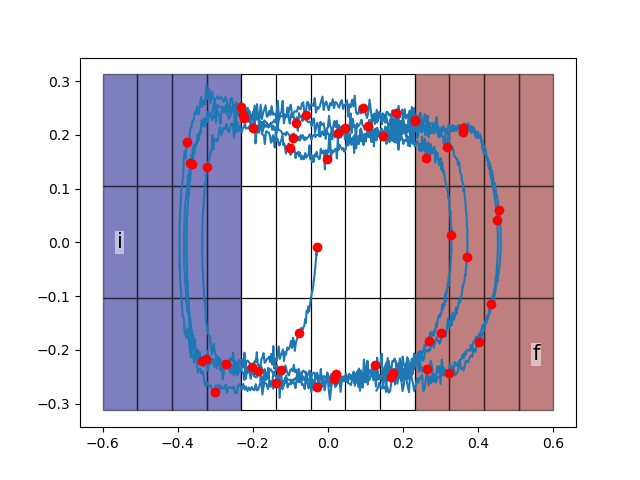
\includegraphics[width=0.9\linewidth]{double_1D}
	  	\caption{Trajectory in the 2D environment.}
	  	\label{double_1D}
  \end{minipage}
	\begin{minipage}[b]{0.5\textwidth}
  		\centering
  		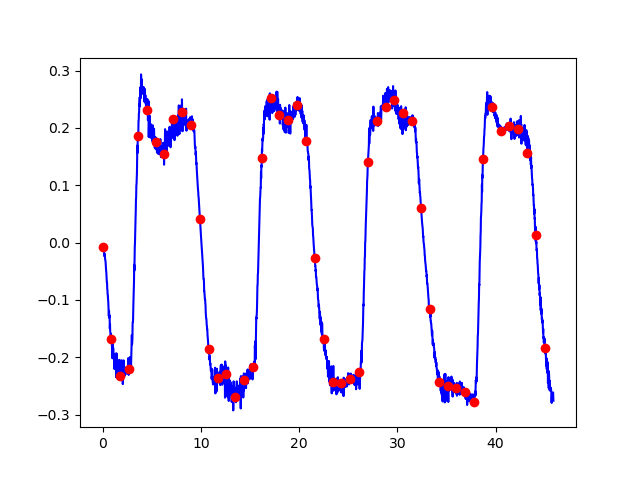
\includegraphics[width=0.9\linewidth]{double_1D_vel}
	  	\caption{Velocity profile.}
	  	\label{double_1D_vel}
  \end{minipage}
  \caption{Trajectory and velocity profile of the double integrator model. The agent is trying to achieve 'go infinity often to i and go infinity often to f'.}
\end{figure}

%% SELF LOOPS ON THE VELOCITY AXIS
The discretization of the state space is chosen to allow self loops during the steady states.
Regardless of the escape time property for the second integrator model, the self loops are not acceptable during transient state. If the transient state evolution is not observed in the case of the second integrator then the abstraction will be stuck in the transient state which make the abstraction not controllable.
\comment{plot the noise}

In figure \ref{double_1D_vel}, the position of the agent at $x \approx -0.3m$ is clearly going backward at the next timestep (the next position of the agent is $x^+ \approx -0.4m$) even if the control is equal to $v_{ref} = 0.2m.s^{-1}$.
In the case of models with no memories ($\Ninputs = 0$),
the abstraction will not be controllable: any state would have a transition going in the opposite direction of the reference velocity (which means that there is no plan solution for bringing the quad from one area to another).
A solution would be to increase the sampling time so that the transient state of the model is more damped after one transition of the model.
However it is not always possible, especially in small environments.
By adding 1 memory ($\Ninputs=1$), the transient state (that cause the backward transition) can be differentiated from the steady states thanks to the memory.
In the next parts, we will show the 2 models.


%% Justification that this model is relevant
In our setup, the timing constants of the unobserved system is $\tau_r = {\nicefrac{1}{k} = 0.5s}$.
This is relevant to use input memories when the sampling time of the planner is close to this value ${\dt \approx 0.5s}$.
For higher sampling time ($\dt \gg 0.5s$) the single integrator model ($\Ninputs=0$) is more relevant as the transient state effect will be completely vanished after $\dt$.
For other cases, abstraction must be investigated individually. Choosing a model with $\Ninputs$ memories, all self loops due to transient states that last less than $(\Ninputs + 1) \dt$ will be removed.


% Talk about the fact that it is not really a double integrator but a double integrator with integral action
% this why it is better working withthe Dnu=1
\comment{I would like to show that if we add the modelling of the integral action, then we can show that the second integrator model is way worst than the reduced abstraction for the same noise model.
Basically, I need to consider the system with the integral action and try to see how I can transform it to find the same model than before but with noise instead.
I need to obtain 2 bodes plots, one for the double integrator model with noise modelled in the dbl int and the other one for the reduced model when there is the int feedback. Really important: have the same noise representation otherwise I cannot compare the bodes.
I should have more noise allowed for the reduced model. Problem: it is not as monotone as before. Can I compose 2 systems? on with what I had before (without the int feedback), another one with the new system added by the integral (I had some troubles with the inputs as the bounds are now supposed to change).}

\subsection{Model with $\Ninputs= 1$ memory}
\begin{figure}[!ht]
	\begin{minipage}[b]{0.5\textwidth}
  		\centering
  		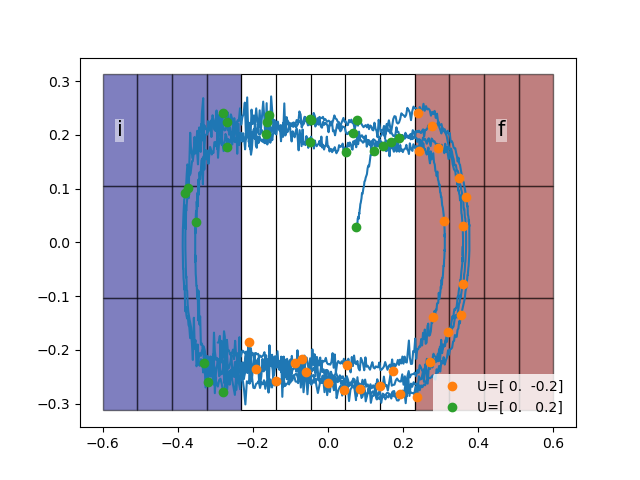
\includegraphics[width=\linewidth]{double_reduced_1D}
	  	\label{double_reduced_1D}
  \end{minipage}
	\begin{minipage}[b]{0.5\textwidth}
  		\centering
  		\includestandalone[width=\linewidth]{speed_plots_reachables_sets}
	  	\label{double_reduced_1D_vel}
  \end{minipage}
  \caption{Trajectory and velocity profile of the double integrator 1-input memory model. The agent is trying to achieve 'go infinity often to i and f'.}
\end{figure}

\begin{figure}[!ht]
  	\centering
	\includestandalone[width=\textwidth]{noise_plot}
  	\label{double_reduced_1D_noise}
  	\caption{The admissible noise of the abstraction have higher magnitudes for the high frequencies. The first plot correspond to the trajectory of the quad, the second is a plot of the noise (plain line) with noise upper and lower bounds (in simple dashed lines) and the upper and lower noise bounds used in the model (double dashed line).}
\end{figure}


%% Overlaps
Figure \ref{double_reduced_1D_vel} shows the profile of the velocity. As we have been noticing in the section on the simulation, there exist overlaps in the discretization on the velocity state.
This overlaps should be noted only for their capacity to cover a wider volume of the state space without increasing the number of symbols. The equivalent discretization would have 5 cells. 

%% NOISE
% the noise is bigger than the modelled noise
As we can see on the figure \ref{double_reduced_1D_vel} and \ref{double_reduced_1D_noise} the noise is higher than the noise modelled. However, this does not affect the correctness of the model as noises of high frequencies can have a higher magnitude.
In the case of the second integrator model, any noise sequence with higher frequency might bring the model to take a non-existent transition.


%% Size of the abstraction

%% Conclusion size of the abstraction

\subsection{Model with $\Ninputs=0$ memory} \label{sec:single_int}

\comment{Show the generated plans!}

This model is equivalent to the single integrator model.
We have been illustrating the advantages of self loops by doing one experiment with self loops and another experiment without self loops.
The FTS created without self loops needs to have a much finer discretization of the state space.
Whereas in the FTS with self loops, the constraint on the minimal size of the state space discretization is only that the transient state on the velocity must counteract the effect of the noise.

% Noise
The sampling time ($\dt \approx 2.0$ for the model with self-loops) is greater than the time constants of the system.
The admissible noise is not that different than the modelled noise.


\begin{figure}[!ht]
	\begin{minipage}[b]{0.5\textwidth}
  		\centering
  		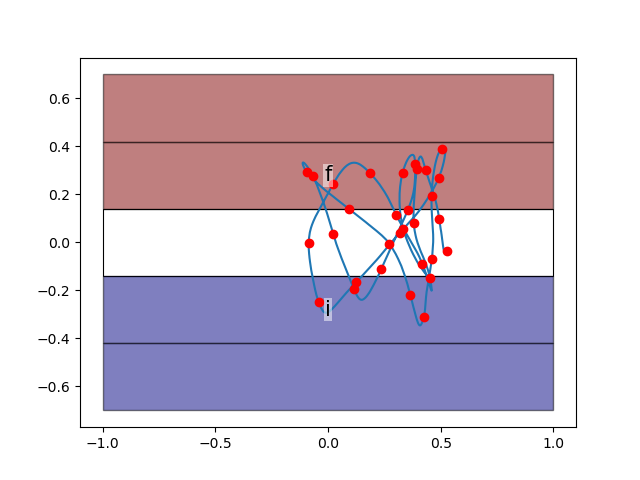
\includegraphics[width=0.9\linewidth]{simple_1D}
	  	\label{simple_1D}
  \end{minipage}
	\begin{minipage}[b]{0.5\textwidth}
  		\centering
  		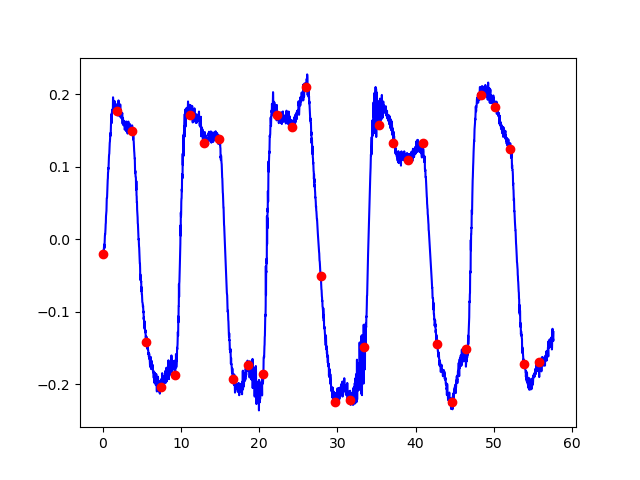
\includegraphics[width=0.9\linewidth]{simple_1D_vel}
	  	\label{simple_1D_vel}
  \end{minipage}
  \caption{Trajectory and velocity profile of the simple integrator model with self loops. The agent is trying to achieve 'go infinity often to i and f'.}
\end{figure}

\begin{figure}[!ht]
	\begin{minipage}[b]{0.5\textwidth}
  		\centering
  		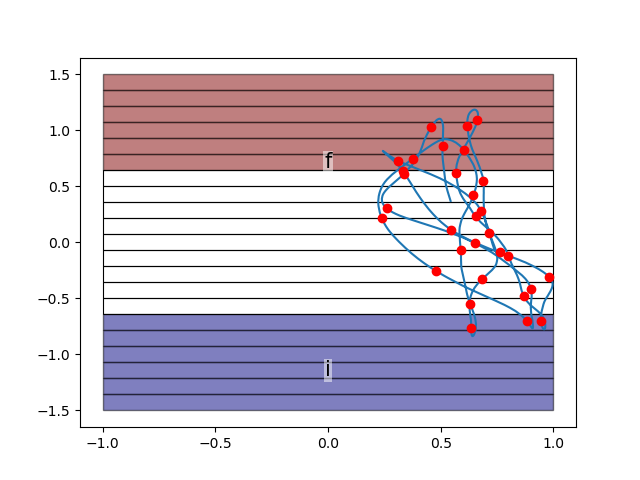
\includegraphics[width=0.9\linewidth]{simplenosl_1D}
	  	\label{simplenosl_1D}
  \end{minipage}
	\begin{minipage}[b]{0.5\textwidth}
  		\centering
  		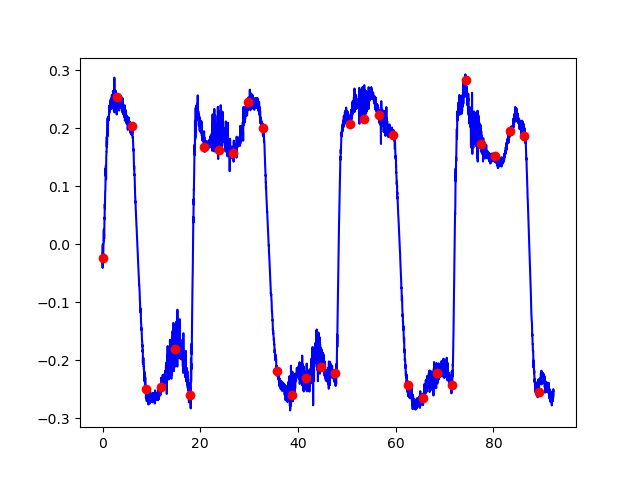
\includegraphics[width=0.9\linewidth]{simplenosl_1D_vel}
	  	\label{simplenosl_1D_vel}
  \end{minipage}
  \caption{Trajectory and velocity profile of the simple integrator model without self loops. The agent is trying to achieve 'go infinity often to i and f'.}
\end{figure}

\subsection{Comparison of the two results}
\comment{
\begin{itemize}
\item compute the branching factor, the precision etc...
\end{itemize}
}

Try to do it for different $\Delta n_u$, show that it does decrease the complexity for $\Delta n_u = 1$. Talk about the case $\Delta n_u = 0$ which correspond to the single integrator case (see part \ref{sec:single_int}).

Comparison to the double integrator case, show how the noise is evolving. Compare the size of the successors between the case where the discretization of the unobserved state (velocity in this case) is lower than the steady state of the unobserved state for a stable sequence. Basically, in one case, the size of the successors is growing (expansion of the successors) in the input memory approach, the size of the successors is reducing (but is bigger than the other one).


\comment{Try to show the 2 abstractions on top of each other to visualize what happened after the reduction}.


\subsection{Discussion over the different models}
The choice of the abstraction will mainly depends on the problem definition.
As we have seen, the sampling time of the process is usually constraint by the environment, the property to verify, and the dynamic process. Small environment will demand to be closer (in time and in space) to the low level controller. This means that the discretization of the state space will have to be small (compared to the environment) and a small sampling time (compared to the time constants of the dynamical system).

Compared to the "raw" model (without memory), the abstraction with extended state could reduce the size of the finite transition system while keeping consistency of the model.
For the "raw" abstraction, the only way to distinguish the transient state is to increase the discretization of the velocity axis. This comes at the price of an higher complexity. Especially in the case of the strong cyclic planner, where the size of the fixed points have a severe impact on the computation of the plans.
In the case of the extended state abstraction, the memories help us to discriminate the transient states that last less than $(\Ninputs+1)\dt$.
This has been an asset in case of small environment.

The admissible noise sequences are bigger (in inclusion sense) than the modelled noise. This come from the computation of the reachable sets which correspond to over approximation of the unobserved dynamics.
However, interesting results usually happens when the unobserved dynamics are slower than the sampling rate.
In this case, the noise can have a higher magnitude at for high frequency than the initially modelled noise.
\comment{This can be seen as a bigger noise set or as unmodelled dynamics. In the case of the quadricopter, the integral action of the speed feedback does not affect the abstraction with extended state as its impact is mainly covered by the bigger admissible noise modelling.}

OVERLAPPS